\documentclass[10pt, twocolumn]{article}
\usepackage[margin=1in]{geometry}                % See geometry.pdf to learn the layout options. There are lots.
\geometry{letterpaper}                   % ... or a4paper or a5paper or ... 
%\geometry{landscape}                % Activate for for rotated page geometry
%\usepackage[parfill]{parskip}    % Activate to begin paragraphs with an empty line rather than an indent
\usepackage{graphicx}
\usepackage{amssymb}
\usepackage{epstopdf}
\usepackage{subfigure}
\usepackage{url}
\DeclareGraphicsRule{.tif}{png}{.png}{`convert #1 `dirname #1`/`basename #1 .tif`.png}

\title{Analyzing Encrypted Web Traffic with Single- and Multi-Class SVMs}
\author{Emily Stark}
\date{\today}                                          % Activate to display a given date or no date

\begin{document}
\maketitle
%\section{}
%\subsection{}

\abstract{
In this project, I applied SVMs to the problem of determining the source of 
encrypted web traffic, without seeing the content or destination of the 
traffic. One of my main goals was to show that a proposed defense against 
traffic analysis can be defeated by a multiclass SVM. I generated two data sets,
and I trained and ran 
one-vs-one and one-vs-all multiclass SVMs on these data sets. 
I implemented a Crammer-Singer
multiclass SVM, anomaly detection via a single-class SVM, and $k$-fold cross-validation 
to tune parameters of all the classifiers. Along the way I designed and 
implemented a custom feature extraction algorithm that uses one of my data sets 
to extract features for the other.
}

\section{Introduction}
Web users, especially those in regions with censored 
Internet access, often use encryption in conjunction 
with anonymizing proxies to conceal which website 
they are visiting. For example, a user whose government 
restricts access to \texttt{https://www.facebook.com} can choose a 
proxy in an uncensored region, and use that proxy to 
forward encrypted HTTP requests and responses to and 
from Facebook. In theory, the censoring entity cannot determine from 
the user's encrypted traffic that the user is visiting 
Facebook. However, encryption does not conceal the direction, 
size, and timing of the packets that a user's web browsing 
generates. In practice, this small amount of information can 
be enough to determine the website that the user is visiting.

This problem is naturally phrased as a supervised learning 
problem. We train on a set of packet traces, where each trace is labelled 
with the website that a user visited to generate it. Given a new,
unlabeled trace, we would 
like to determine the website that a user visited to generate this trace.
 The point of training such a classifier is not 
necessarily to make it easier for a censor to do its job, but rather 
to understand the security guarantees that a user gets from using 
an anonymizing proxy to forward encrypted web traffic, as well as 
the effectiveness of proposed defenses against traffic analysis. 
One such proposed defense is to generate a background request to a 
random website for every encrypted request to a sensitive website~\cite{torfingerprinting}. 
This defense, which I will refer to as the random-visit defense, 
attempts to confuse the classifier by the addition of random 
noise to the traffic generated by a visit to a sensitive website.

In this project, I applied support vector machine (SVM) classifiers 
to the problem of determining the source website of a stream of 
encrypted web traffic. My goals were 1.) to train a SVM to 
effectively classify traces of encrypted packets into their source 
websites, and 2.) to show that SVMs can be used to break the random-visit 
defense described above. While SVMs have been used before for 
encrypted traffic analysis~\cite{torfingerprinting}, the random-visit defense 
is a very recent proposal and has not been well-studied yet.

Previous work classifies encrypted traffic analysis into two settings: 
closed world and open world. In the closed world setting, we assume that 
the user visits one of a small number of websites over an encrypted, 
anonymized connection, and the censor wishes to determine which website 
the user is visiting. In the open world problem, which is much harder, the 
censor has a small list of offensive websites that it wishes to block, but 
the user might visit any website on the Internet. The censor wishes to 
recognize when the user is visiting one of the offensive websites, and which 
of the offensive websites is being visited. I used SVM-based techniques to 
perform traffic analysis in both a very small closed-world setting and an 
open-world setting.

Below I summarize the tasks that I completed for this project.
\begin{itemize}
\item \textbf{Data generation and preprocessing.} I generated packet 
traces of visits to HTTPS websites, both with and without random 
background visits. From these traces, I generated a feature vector for 
each visit. This process is described in more detail in Section~\ref{sec:data}. 
\item \textbf{Training binary and multiclass SVMs.} I used the 
generated data to train several types of SVMs from the Python scikits-learn 
library~\cite{sklearn}. These included a binary SVM, as well as one-vs-all
and one-vs-one multiclass SVMs based on a binary SVM. I implemented $k$-fold cross-validation 
to determine the SVM parameters.
\item \textbf{Implementing a multiclass SVM and a single-class SVM for anomaly detection.} 
I built a multiclass SVM using the Python \texttt{cvxopt} library~\cite{cvxopt}.
 To investigate the 
open-world setting, I also built and trained a single-class SVM to perform 
anomaly detection.
\item \textbf{Designing and implementing a custom dimensionality reduction algorithm.} 
Because \texttt{cvxopt} does not scale to very large problems~\cite{cvxoptscale}, the feature vectors from the 
packet traces were too large to run on the multiclass and single-class SVMs that I built. 
I designed a feature selection algorithm (Section~\ref{sec:dimred}) similar to mutual information 
that uses data from website visits without the 
random-visit defense to select features for the data generated using the random-visit defense.
\end{itemize}

All the code that I wrote for this project is available online~\cite{github}.

\section{Related work}

Much previous work has analyzed encrypted traffic to reveal the destination website or 
even uncover sensitive information entered by the user on a HTTPS website. Early
approaches simply fingerprinted websites by recording the sizes of objects generated 
by a visit to the website~\cite{safeweb}. Since then, various machine learning 
and data mining techniques, such as Jaccard coefficients and multinomial naive Bayes classifiers,
have been applied to the encrypted traffic analysis problem~\cite{herrmann,liberatore}. 
A recent work showed that SVMs are an effective traffic analysis technique~\cite{torfingerprinting}, even 
against protocols such as Tor (an anonymity network) that employ pipelining, which makes 
traffic analysis more difficult. This work proposed the random-visit defense discussed above. In 
this project I investigated the effectiveness of the random-visit defense in analyzing 
SSL-encrypted web traffic.

\section{Data generation and preprocessing}
\label{sec:data}

In this paper, I will refer to a \textit{target site} as one of the HTTPS websites that a censoring 
entity wants to block, and that a user tries to visit via an anonymizing proxy.
 The target site is the label in the classification 
problem. The \textit{background site} is the random website loaded in the background when a 
user is using the random-visit defense.

I generated two data sets for this project. The \textit{single-visit} data set consists of packet 
traces from individual visits to a small set of target sites. The \textit{multi-visit} data set 
consists of packet traces from individual visits to a small set of target sites, where each visit 
happened concurrently with a visit to a random background site.

I used 8 popular HTTPS websites (two banks, two file sharing applications, two social networks, 
Google, and the Tor website) as target sites. The list of websites is located in \texttt{gen\_data.py}.
In future, this work could be made much more convincing by increasing the number of target sites 
to several hundred, but for this project I limited the closed-world setting to a few websites 
because of limited computational resources. (I ran all experiments on my Macbook Pro laptop, and 
for some classifiers, even with the small list of target sites, I had to limit the amount of data 
used in training in order to not run out of memory. I discuss this limitation in greater detail 
in Section~\ref{sec:multiclassimplementation}.)

The background sites were chosen randomly from a list of 5000 of the most popular websites~\cite{alexa}. 
While the background sites were visited over HTTP, I only used information such as packet timings and 
lengths that would be available if HTTPS background sites were used. A real deployment of the 
random-visit defense would use HTTPS-enabled sites as background sites; I only used HTTP sites as 
background sites in this project because a large list of HTTPS websites was not readily available.

\subsection{Data generation}

For the single-visit data set, I wrote a Python script (\texttt{gen\_data.py}) to visit each site 
in the list of target sites 30 times and record a packet trace with \texttt{tcpdump}. Each visit 
occurred in a new instance of Google Chrome (in incognito mode, to prevent the browser from 
using cached resources in subsequent visits).

For the multi-visit data set, I modified \texttt{gen\_data.py} to, on each target site visit, 
simultaneously open a second tab and load a randomly selected background site in that tab. For the 
multi-visit data set, I recorded 60 visits to each target site instead of 30, since the multi-visit 
data set presents a harder classification problem and therefore having more training data is helpful.

\subsection{Preprocessing packet traces into feature vectors}
\label{sec:preprocessing}

\texttt{preprocess.py} uses \texttt{tcpdump} to parse the raw packet traces, and then translates 
each target site visit into a feature vector. I defined three features for each recorded packet: the 
time relative to the time of the first packet in the trace, the direction of the packet (to or from 
the user's machine), and the length of the packet. I padded each vector with $-1$ values so that all 
feature vectors in each data set were the same length. This selection of features led to large vectors 
with several thousand features. For the classifiers that were unable to handle such large feature vectors 
(my implementations of a multiclass SVM and a single-class SVM for anomaly detection, both using 
\texttt{cvxopt}), I designed and implemented a dimensionality reduction algorithm that I describe in 
Section~\ref{sec:dimred}.

\section{SVMs in the closed world setting}

For the closed world setting, I compared three multiclass SVMs:
\begin{itemize}
\item a one-vs-one multiclass SVM implemented in the scikits-learn library,
\item a one-vs-all multiclass SVM implemented in the scikits-learn library,
\item a multiclass SVM that I implemented using \texttt{cvxopt} (the implementation is 
described in Section~\ref{sec:multiclassimplementation}).
\end{itemize}

I investigated the performance of these SVMs on both the single-visit and multi-visit data. 
The training data was a list of feature vectors, where each feature vector corresponds to a 
packet trace from a visit to a target site, as described in Section~\ref{sec:preprocessing}.

I implemented $k-$fold cross-validation for each SVM to choose parameters. I also used 
cross-validation to observe how a classifier's performance improves with the addition of more data 
and how it suffers when more classes are introduced. Data from the cross-validation process is shown 
in Section~\ref{sec:crossvalidation}.

In the closed-world setting, I used linear kernels for all three types of multi-class SVMs.
I briefly explored using the radial basis function as a kernel in the one-versus-one multiclass 
SVM, but I could not find parameters that outperformed the linear kernel. For example, using $k$-fold 
cross-validation with $k=6$ and the full dimensionality multi-visit data with 30 visits per target site, the best choice of 
parameters that I was able to find for the linear and RBF kernels led to average performance of about 
$30\%$ correct for both kernels. Assuming that I didn't miss some better choice of parameters for the 
RBF kernel, this result suggests that the data is mostly linearly separable with outliers: the RBF kernel 
does no better than the linear kernel, and it can do worse by overfitting.

\subsection{Multiclass SVM implementation}
\label{sec:multiclassimplementation}

I implemented the primal form of the Crammer-Singer multiclass SVM~\cite{cramersinger} using the Python \texttt{cvxopt} 
library for convex optimization. The implementation can be found in \texttt{multiclass\_svm.py} in 
the Github repository for this project.

One of the unanticipated challenges of this part of the project was that, on my laptop, \texttt{cvxopt} 
consistently ran out of memory when solving the multiclass SVM for the full-dimensionality multi-visit data
(which consists of 60 visits per target site). To save memory, I wrote all the training data to disk and 
read out one vector at a time, but using \texttt{cvxopt} still requires keeping large coefficient 
and constraint matrices in memory. To use my multiclass SVM implementation, I had to reduce the size of the 
data to 30 visits per target site and also perform dimensionality reduction. While my dimensionality 
reduction turned out to improve classification performance, the memory limitations meant that I couldn't 
compare the multiclass SVM's performance on reduced dimensionality data to its performance on full 
dimensionality data, or to other SVMs' performance on full dimensionality data.

\subsection{Cross-validation for parameter tuning}
\label{sec:crossvalidation}
\begin{figure}
\begin{center}
\subfigure[One-vs-one SVM performance as the number of visits to each of the 8 target sites varies.]{
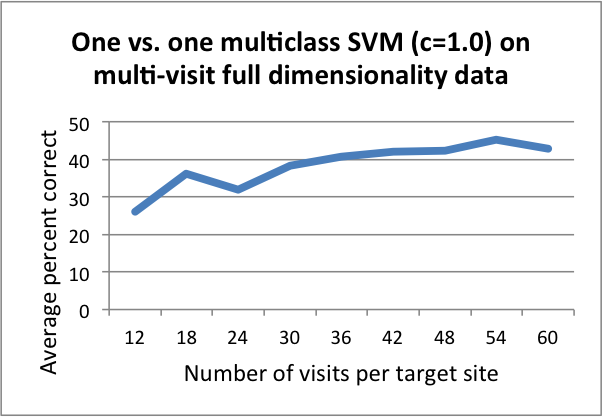
\includegraphics[scale=0.6]{graphs/1v1_vary_data.png}
\label{fig:vary-visits}
}
\subfigure[One-vs-all SVM performance as the number of target sites varies. There are 30 visits to each target site.]{
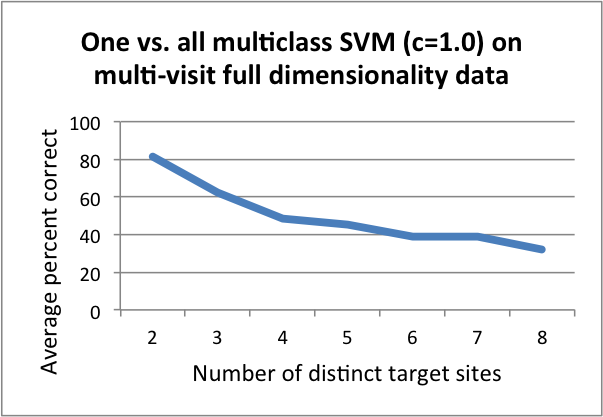
\includegraphics[scale=0.6]{graphs/1vall_vary_labels.png}
\label{fig:vary-labels}
}
\caption{$k$-fold cross-validation results (with $k=6$) as the amount of training data increases, 
 with $c=1.0$. The training data is the multi-visit data set with 
no dimensionality reduction.}	
\end{center}
\label{fig:vary-amt}
\end{figure}

\begin{figure*}
\begin{center}
\subfigure[Single-visit data with full dimensionality.]{
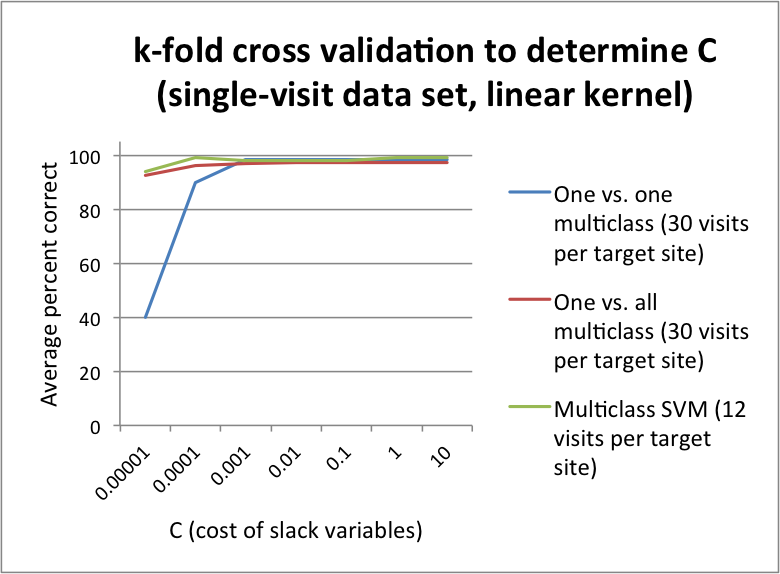
\includegraphics[scale=0.6]{graphs/single_visit_c.png}
\label{fig:kfoldc-single}
}
\subfigure[Multi-visit data with dimensionality reduced to 50 features.]{
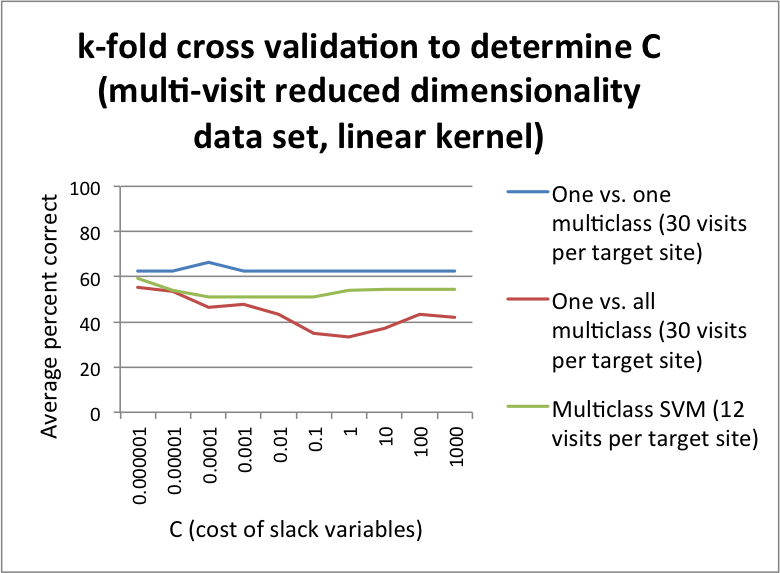
\includegraphics[scale=0.6]{graphs/multi_visit_c.png}
\label{fig:kfoldc-multi}
}
\caption{$k$-fold cross-validation results (with $k=6$) for tuning $c$, the cost associated with 
each slack variable. The smaller size of the training data for the multiclass SVM is due to 
limited computational resources.}
\label{fig:kfoldc}
\end{center}
\end{figure*}


I implemented $k$-fold cross-validation to determine parameters of each SVM, and also to study how 
SVM performance changes as the amount of training data increases. Figure~\ref{fig:vary-visits} shows how the 
one-vs-one multiclass SVM performance increases with the number of samples for each target site. As we expect,
performance increases somewhat linearly with the amount of training data. Figure~\ref{fig:vary-labels} shows 
how one-vs-all multiclass SVM performance deteriorates as the number of classes increases. Though it is difficult 
to extrapolate from the graph, we see a large fall in performance as the number of classes grows from $2$ to $4$, 
and then a slight leveling off. Hopefully, this means that the classifier's performance scales well with the 
number of classes and that these results are transferrable to a more realistic closed-world setting with dozens or 
hundreds of target sites.

Figure~\ref{fig:kfoldc} shows how all three multiclass SVMs perform as $c$, the cost associated with each slack 
variable, varies. On the single-visit data set, each SVM has a clear peak for the values of $c$ that I used in the 
experiment. After hitting the peak for the single-visit data, the performance does not seem to change much with 
increasing $c$. This indicates that there is always some number of points that must be misclassified by a certain amount, 
since increasing $c$ does not change the performance of the classifier. For the multi-visit data, choosing $c$ is not 
as clear-cut: for example, in the multiclass SVM, values of $c$ as low as $0.000001$ and as high as $1.0$ appear to be 
good choices.


\subsection{Performance results and analysis}


Tables~\ref{tab:singleperf} and~\ref{tab:multiperf} show how the three multi-class SVMs perform on the single- and multi-visit data. 
The one-vs-one multiclass SVM consistently slightly outperforms the one-vs-all SVM, both on single- and multi-visit data, with and without dimensionality reduction. The classifiers perform very well on the single-visit data, and they achieve almost $70\%$ accuracy on 
the multi-visit data. With 30 visits per target site and the feature vectors reduced to 50 dimensions, the multiclass classifier
outperforms the one-vs-all and one-vs-one classifiers.

\begin{table}
\caption{Classification performance for the single-visit data set on two multiclass SVMs. (The third multiclass SVM that 
I implemented runs out of memory on full-featured data, and my dimensionality reduction algorithm only works on 
the multi-visit data set.) Half the data 
is used for training and half for testing. There are $30$ visits per target site.}
\begin{center}
\begin{tabular}{|c|c|r|}
\hline
SVM & $c$ & Percent correct \\ \hline
One-vs-one &$0.01$ & $97\%$ \\ \hline
One-vs-all &  $0.0001$ & $94\%$ \\ \hline
\end{tabular}
\end{center}
\label{tab:singleperf}
\end{table}%

\begin{table*}
\caption{Classification performance for the multi-visit data set on three multiclass SVMs, with and without 
dimensionality reduction. Half the data 
is used for training and half for testing. Original features means that no dimensionality reduction was 
performed on the data.}
\begin{center}
\begin{tabular}{|c|c|c|r|r|}
\hline
SVM & Features & Visits per target site & $c$ & Percent correct \\ \hline
One-vs-one & original & 60 & $0.0001$ & $36\%$ \\ \hline
One-vs-one & 50 & 60 & $0.0001$ & $69\%$ \\ \hline
One-vs-one & 50 & 30 & $0.0001$ & $48\%$ \\ \hline
One-vs-all & original & 60 & $0.000001$ & $33\%$ \\ \hline
One-vs-all & 50 & 60 & $0.000001$ & $64\%$ \\ \hline
One-vs-all & 50 & 30 & $0.000001$ & $52\%$ \\ \hline
Multiclass & 50 & 30 & $1.0$ & $54\%$ \\ \hline
\end{tabular}
\end{center}
\label{tab:multiperf}
\end{table*}%


In this small closed-world setting, therefore, the random-visit defense is not effective. While random background 
requests do confuse a classifier trained on single-visit data, dimensionality reduction can be used to train a classifier that 
distinguishes a target site in spite of random noise added to the packet trace. The reason for this, as I discuss in Section~\ref{sec:dimred}, is that the dimensionality reduction algorithm uses the single-visit data set to extract features for the multi-visit 
data set. This may not be an unrealistic scenario: for example, a censoring entity might collect single-visit data during a time 
period in which target sites are not blocked, and then use this data to extract features for multi-visit data that is generated 
when target sites are blocked and users are employing the random-visit defense.

\section{A single-class SVM for the open world setting}

For the open world setting, I implemented the dual form of a single-class SVM with kernels, using the 
\texttt{cvxopt} library. This implementation can be found in \texttt{anomaly\_detection.py}. For each target site, I trained 
a separate anomaly detector to recognize visits to that site as positive events, in hopes that visits to any other site 
would register as negative events, thereby enabling the detection of visits to target sites. Unfortunately, the single-class
SVM proved to be of little utility in this setting. Because of \texttt{cvxopt}'s memory limitations, I could only run the 
anomaly detector on dimensionality-reduced multi-visit data. As in the closed-world setting, I performed $k$-fold cross 
validation to tune the parameters, but I was unable to find a set of parameters for either a linear or RBF kernel that resulted 
in a high true-positive/true-negative rate and a low false-positive/false-negative rate. In this application, a low true-positive 
rate might be acceptable if the false-positive rate is also low: a censoring entity probably does not want to disrupt a large 
percentage of Internet traffic because it has registered as a false positive on an anomaly detector for a target site, but an 
anomaly detector that allows a censor to discover a small percentage of target site visits without disrupting other traffic 
might be desirable. I therefore tuned the parameters for low false positive rates, and with an RBF kernel with $\beta=0.0000005$, $v=0.01$, and multi-visit data with 30 visits per target site, reduced to $130$ dimensions, the anomaly detector obtained an average true positive 
rate of $15\%$ with an average false positive rate of $4\%$. In future, I would like to experiment with the minimum enclosing ball 
anomaly detector to determine if that model better fits this data.

\section{Dimensionality reduction}
\label{sec:dimred}

Partly for fun, and partly out of a lack of knowledge as to what dimensionality reduction algorithm would be appropriate for this data, I 
designed and implemented a custom feature extraction algorithm to use on the multi-visit data. My motivation for constructing a custom 
algorithm came from two characteristics of the original multi-visit feature vectors:
\begin{itemize}
\item Because each feature vector represents a packet trace with random background packets inserted into it, a simple 
feature ranking does not suffice. The importance of feature $i$ in vector $x_{1}$ is only very loosely correlated with the 
importance of feature $i$ in vector $x_{2}$: in $x_{1}$, feature $i$ could come from a packet originating at the target site, 
whereas in $x_2$, feature $i$ could very easily correspond to a packet originating from a random background site.
\item I wanted to take advantage of the existence of the single-visit data to select features for the multi-visit data. 
Intuitively, the existence of single-visit feature vectors for each target site provides a lot of information about what 
features in a multi-visit data point are relevant to the target site.
\end{itemize}

The algorithm I implemented can be found in \texttt{dim\_reduction.py} in the project repository. The assumption made by this method 
is that packets from the random background visit are uniformly dispersed throughout a multi-visit packet trace. For example, if a packet 
of length $m$ is sent in the middle of a single-visit trace to \texttt{https://encrypted.google.com}, then we assume that it is 
likely that a packet of length $m$ is sent in the middle of a multi-visit trace to \texttt{https://encrypted.google.com} and a random
background site. To use this assumption, the algorithm ranks each packet in each multi-visit feature vector according to how similar 
this packet is to packets in similar positions in each of the single-visit feature vectors.

The feature extraction algorithm is parameterized by $b$, a number of blocks, and $\epsilon$, a window around packet lengths.
The algorithm is given as input a multi-visit feature vector $x$, a matrix of single-visit vectors $X$, and a desired number of 
features $n$. To produce a dimensionality-reduced version of $x$ with $n$ features, the algorithm does the following:
\begin{enumerate}
\item Divide $x$ into $b$ blocks.
\item For each packet $p$ in $x$:
\begin{enumerate}
\item $Score(p) \leftarrow 0$
\item $i \leftarrow $ the index of the block that contains $p$
\item For each vector $x' \in X$:
\begin{enumerate}
\item Divide $x'$ into $b$ blocks.
\item $bx' \leftarrow $ the packets in the $i^{th}$ block of $x'$
\item $Score(p) \leftarrow Score(p) + \frac{k}{m}$, where $k$ is the number of packets in $bx'$ with the same direction as $p$ and with a length within $\epsilon$ of the length of $p$, and $m$ is the total number of packets in $bx'$ with the same direction as $p$.
\end{enumerate}
\end{enumerate}
\item Return $x_{new} \leftarrow $ the vector with a feature for the length and direction of each of the $n$ distinct highest scoring packets
\end{enumerate}

In short, the algorithm scores each packet of each vector according to how similar it is to packets in the corresponding blocks of
single-visit feature vectors. Different features are chosen for different vectors. The feature extraction depends only on the 
single-visit data set, not on other multi-visit data points or on the labels. This algorithm is akin to mutual information, except 
that it operates on packets instead of individual features, and it compares each feature to features in similar regions of 
single-visit feature vectors instead of to the corresponding feature in other multi-visit algorithms.

In my implementation, I precomputed the numbers of packets with each length and direction in each block of each single-visit 
feature vector, so that running the algorithm on all the multi-visit feature vectors didn't take more than a few seconds on my 
laptop.

This algorithm seems to lead to good performance on multiclass SVMs, by picking out the few packet lengths/directions that 
distinguish target site visits. I used $\epsilon=100$ and $b=15$, and found these parameters to work well enough.
 In future, I would like to understand more rigorously why this algorithm works, what good choices of parameters are, how 
 this algorithm is similar or dissimilar to mutual information,
  and if there are
existing, well-studied alternatives that perform the same type of feature selection.

Table~\ref{tab:dimred-kfold} shows a SVM's performance as the number of features varies. The dimensionality 
reduction algorithm definitively increases performance over the original feature vectors, and performance 
seems to improve as the number of features gets smaller. This suggests that there are a small number of 
packets that distinguish each target website, and the dimensionality reduction algorithm is effective at 
extracting these features while removing noise.

\begin{table}
\caption{$k$-fold cross-validation performance of a one-vs-one multiclass SVM as the dimensionality of 
the data is varied. $c$ is fixed at $1.0$ and $k$ is fixed at $6$. The data is the multi-visit data set 
with 30 visits to each target site.}
\begin{center}
\begin{tabular}{|r|r|}
\hline
Number of features & Average percent correct \\
\hline
30 & 69\% \\
\hline
50 & 61\% \\
\hline
70 & 59\% \\
\hline
90 & 60\% \\
\hline
110 & 59\% \\
\hline
All original features & 36\% \\ \hline
\end{tabular}
\end{center}
\label{tab:dimred-kfold}
\end{table}%

\section{Conclusions}

In this project, I investigated the performance of several single- and multiclass SVMs on packet traces from visits to encrypted websites. 
I found that the recently proposed random-visit defense against traffic analysis does not hold up, since a SVM trained on 
dimensionality-reduced multi-visit data can achieve up to $70\%$ accuracy against this defense. In the future, I would like to better 
understand the feature extraction algorithm that I designed from a rigorous standpoint, and also study how to improve anomaly detection 
for the open-world setting of the encrypted traffic analysis problem.


\bibliography{paper}
\bibliographystyle{plain}


\end{document}  